%% Modified by James Saunderson to comply with thesis requirements for Monash University.
%%
%% Modified by Ricardo Garcia-Rosas to satisfy the rules established by the University of Melbourne's Research Higher Degrees Committee as of 4th of June 2019.
%% Guidelines can be found at: https://gradresearch.unimelb.edu.au/__data/assets/pdf_file/0004/2027839/Preparation-of-GR-theses-rules.pdf
%%
%% ----------------------------------------------------------------
%% Thesis.tex -- MAIN FILE (the one that you compile with LaTeX)
%% ----------------------------------------------------------------

% Set up the document
\documentclass[a4paper, 11pt, oneside]{Thesis}  % Use the "Thesis" style, based on the ECS Thesis style by Steve Gunn
%
% Put your figures in this directory
\graphicspath{Figures/}  % Location of the graphics files (set up for graphics to be in PDF format)
%

% Include any extra LaTeX packages required
\usepackage[square, numbers, comma, sort&compress]{natbib}  % Use the "Natbib" style for the references in the Bibliography
\usepackage{verbatim}  % Needed for the "comment" environment to make LaTeX comments
\usepackage{array} % for the table on page v.
\usepackage{multirow} % for the table on page v.
\usepackage{multicol} % for the table on page v.
\usepackage[table]{xcolor} % for the table on page v.
\usepackage{vector}  % Allows "\bvec{}" and "\buvec{}" for "blackboard" style bold vectors in maths
\usepackage{pdfpages} % allows entire pdf files to be included in the document (for thesis including published works)
\hypersetup{urlcolor=blue, colorlinks=true}  % Colours hyperlinks in blue, but this can be distracting if there are many links.

%% ----------------------------------------------------------------
% include any additional macros here
\newcommand\bcwt[1]{\cellcolor{black}\bfseries\textcolor{white}{#1}} % black cells white text for table on page v.
%% ----------------------------------------------------------------
\begin{document}
\frontmatter      % Begin Roman style (i, ii, iii, iv...) page numbering

%
\UNIVERSITY{{Monash University}}
%
%%%%%%%%%%%%%%%%%%%%%%%%%%%%%%%%%%%%%%%%%%%%%%%%%%%%%%%%%%%%%%%%%%%%%%%%%
% Update your faculty here:
\school{{Faculty of Engineering}}
% update your department/school here
\department{{Department of \ldots}}
% this is the year of submission
\gradtime{{2022}}
% degree the thesis is for (Master of Engineering Science or Doctor of Philosophy)
\degree{Master of Engineering Science}
% degrees currently held by the student
\studentdegree{Student's academic degrees}
%%%%%%%%%%%%%%%%%%%%%%%%%%%%%%%%%%%%%%%%%%%%%%%%%%%%%%%%%%%%%%%%%%%%%%%%%

%
%%%%%%%%%%%%%%%%%%%%%%%%%%%%%%%%%%%%%%%%%%%%%%%%%%%%%%%%%%%%%%%%%%%%%%%%%
% Set up the Title Page
% Change your thesis title and your information here
\title  {Thesis Title}
\authors  {\texorpdfstring
            {\href{your web site or email address}{Author's full name}}
            {Author's full name}
            }

%%%%%%%%%%%%%%%%%%%%%%%%%%%%%%%%%%%%%%%%%%%%%%%%%%%%%%%%%%%%%%%%%%%%%%%%%

\maketitle
%% ----------------------------------------------------------------

\setstretch{1.3}  % It is better to have smaller font and larger line spacing than the other way round

% Define the page headers using the FancyHdr package and set up for one-sided printing
\fancyhead{}  % Clears all page headers and footers
\rhead{\thepage}  % Sets the right side header to show the page number
\lhead{}  % Clears the left side page header

\pagestyle{fancy}  % Finally, use the "fancy" page style to implement the FancyHdr headers

%% ----------------------------------------------------------------
% The copyright Page
% https://www.monash.edu/graduate-research/examination/publication
% https://www.monash.edu/rlo/graduate-research-writing/write-the-thesis
% https://www.monash.edu/rlo/graduate-research-writing/write-the-thesis/writing-the-thesis-chapters/structuring-a-long-text
\copyrightnotice{

% \addtocontents{toc}{\vspace{1em}}  % Add a gap in the Contents, for aesthetics

\emph{Insert one of the following notices.}

\emph{Notice 1}

\textsuperscript{\textcopyright  \authornames (\gradtime).}

\emph{The second notice certifies the appropriate use of any third-party material in the thesis. Students choosing to deposit their thesis into the restricted access section of the repository are not required to complete Notice 2.}

\emph{Notice 2}

\textsuperscript{\textcopyright  \authornames (\gradtime).}

I certify that I have made all reasonable efforts to secure copyright permissions for third-party content included in this thesis and have not knowingly added copyright content to my work without the owner's permission.


}
\clearpage  % copyright ended, start a new page

% https://www.monash.edu/graduate-research/examination/publication
% https://www.monash.edu/rlo/graduate-research-writing/write-the-thesis
% https://www.monash.edu/rlo/graduate-research-writing/write-the-thesis/writing-the-thesis-chapters/structuring-a-long-text
\abstract{
\addtocontents{toc}{}  % Add a gap in the Contents, for aesthetics

\emph{The abstract should outline the main approach and findings of the thesis and must not be more than 500 words.}

}


\clearpage  % Abstract ended, start a new page

%% ----------------------------------------------------------------
% Publications Page 
%% (OPTIONAL)
%% Publications during enrolment
%% ACTION
%%      You may wish to list your publications arising from your research degree enrolment. Otherwise remove this section.
%%      The format of this section is mostly up to you. I have added lists for categorisation by type. You may alter this.
\Publicationslist{{}
Journal Publications\\[-3\parskip]
{\small
\begin{itemize}
	\item \fullcite{example3}
	\item \fullcite{example5}
\end{itemize}
}

Conference Publications\\[-3\parskip]
{\small
\begin{itemize}
	\item \fullcite{example1}
	\item \fullcite{example2}
\end{itemize}
}

Research Data\\[-3\parskip]
{\small
\begin{itemize}
	\item \fullcite{example4}
\end{itemize}
}

%% SYNTAX: \href{ref}{text}
%% NOTE: Escape underscores in the displayed text with \_ (the ref should just be the url, as is)
Free \& Open Source Code\\[-3\parskip]
{\small
\begin{itemize}
	\item \href{https://github.com/Brandon-Johns/crane-dynamics-simulator/}{https://github.com/Brandon-Johns/crane-dynamics-simulator}
\end{itemize}
}

}
\clearpage  % Declaration ended, now start a new page

%% ----------------------------------------------------------------
% Declaration of publications Page required for the Thesis, your institution may give you a different text to place here
%% (REQUIRED) (Thesis including published works only)
%% ACTION
%%      Ensure that your thesis meets the thesis including published works requirements. Some faculties vary requirements in terms of the number of papers required, status of papers and other criteria
%%      Read through and change the details that are in all caps (you should not use all caps in the replacement text)
\Declarationpublication{{}
I hereby declare that this thesis contains no material which has been accepted for the award of any other degree or diploma at any university or equivalent institution and that, to the best of my knowledge and belief, this thesis contains no material previously published or written by another person, except where due reference is made in the text of the thesis.

%% ACTION: Change COUNT, COUNT, THEME, NAME, NAME
This thesis includes COUNT original papers published in peer reviewed journals and COUNT submitted publications.. The core theme of the thesis is THEME. The ideas, development and writing up of all the papers in the thesis were the principal responsibility of myself, the student, working within the \printThesisDepartment under the supervision of NAME and NAME.

%% ACTION: Remove this paragraph for theses with sole-authored work
The inclusion of co-authors reflects the fact that the work came from active collaboration between researchers and acknowledges input into team-based research.

%% ACTION: If this is a laboratory-based discipline, a paragraph outlining the assistance given during the experiments, the nature of the experiments and an attribution to the contributors could follow.

%% ACTION: Insert chapter numbers
In the case of Chapters \ref{chap:article1} and \ref{chap:article2}, my contribution to the work involved the following:

%% ACTION: Update the table to list your publications
%%      The status might be: in press, accepted, returned for revision, submitted
%%      If no co-authors, leave fields blank 
\definecolor{thesisdark}{HTML}{1E1E1E}
\definecolor{thesislight}{HTML}{EEEEEE}
\newcommand{\thesisDPFormatVspace}[1]{\vspace{1ex}{#1}\vspace{1ex}}
\newcommand{\thesisDPFormatH}[1]{\textcolor{thesislight}{\textbf{#1}}}
\newcommand{\thesisDPFormatHv}[1]{\thesisDPFormatVspace{\textcolor{thesislight}{\textbf{#1}}}}
\newcommand{\thesisDPAuthorFirst}[1]{\Block[v-center]{1-1}{\thesisDPFormatVspace{#1}}}
\newcommand{\thesisDPAuthor}[1]{\cline{5-6}&&&&\Block[v-center]{1-1}{\thesisDPFormatVspace{#1}}}
\newcommand{\thesisDPAuthorYN}[1]{\Block[v-center]{1-1}{#1}\\}
\newcommand{\thesisDP}[2]{\Block[v-center]{#1-1}{#2} &}
\newcommand{\thesisDPv}[2]{\Block[v-center]{#1-1}{\thesisDPFormatVspace{#2}} &}
\begin{center}
    \addtolength{\leftskip} {-1cm} %% Fix centering for when table is wider than \textwidth
    \addtolength{\rightskip}{-1cm} %% Fix centering for when table is wider than \textwidth
    \small
    %\footnotesize
    \begin{NiceTabular}[colortbl-like]
            {|c|p{30mm}|c|p{25mm}|p{37mm}|p{25mm}|}
        \hline
        \Block[fill=thesisdark,v-center]{1-1}{\thesisDPFormatH{\makecell{Thesis\\Chapter}}} &
        \Block[fill=thesisdark,v-center]{1-1}{\thesisDPFormatH{Publication Title}} &
        \Block[fill=thesisdark,v-center]{1-1}{\thesisDPFormatH{Status}} &
        \Block[fill=thesisdark,v-center]{1-1}{\thesisDPFormatH{Nature and \% Student Contribution}} &
        \Block[fill=thesisdark,v-center]{1-1}{\thesisDPFormatHv{Co-author name(s) Nature and \% of Co-author's contribution}} &
        \Block[fill=thesisdark,v-center]{1-1}{\thesisDPFormatH{Co-author(s), Monash student}}\\

        %% ACTION: The first argument of \thesisDP must be the total number of co-authors
        %%    i.e. change the number 4 to the number of co-authors
        %%    This defines how big the multi-row block is
        \hline
        \thesisDP{4}{\ref{chap:article1}}
        \thesisDPv{4}{The Title of My First Published Article}
        \thesisDP{4}{Published}
        \thesisDP{4}{(70\%)}
        \thesisDPAuthorFirst{NAME: contribution~1, contribution~2 (10\%)} & \thesisDPAuthorYN{No}
        \thesisDPAuthor{NAME: contribution~1, contribution~2 (10\%)} & \thesisDPAuthorYN{No}
        \thesisDPAuthor{NAME: contribution~1 (5\%)} & \thesisDPAuthorYN{No}
        \thesisDPAuthor{NAME: contribution~1 (5\%)} & \thesisDPAuthorYN{No}

        %% ACTION: The first argument of \thesisDP must be the total number of co-authors
        \hline
        \thesisDP{2}{\ref{chap:article2}}
        \thesisDPv{2}{The Title of My Second Published Article}
        \thesisDP{2}{In Press}
        \thesisDP{2}{(80\%)}
        \thesisDPAuthorFirst{NAME: contribution~1, contribution~2 (10\%)} & \thesisDPAuthorYN{No}
        \thesisDPAuthor{NAME: contribution~1, contribution~2 (10\%)} & \thesisDPAuthorYN{No}
        \hline
    \end{NiceTabular}
\end{center}

I have not renumbered sections of submitted or published papers in order to generate a consistent presentation within the thesis.

\textbf{Student name:} \printThesisAuthor

%% OPTIONAL: Choose how to display the date
%%      For more options, see the package 'datetime'
\ddmmyyyydate
%\yyyymmdddate\renewcommand{\dateseparator}{-}

%% ACTION: Add your signature file
\textbf{Student signature:}\hspace{3mm}%%
\raisebox{-.5\height}{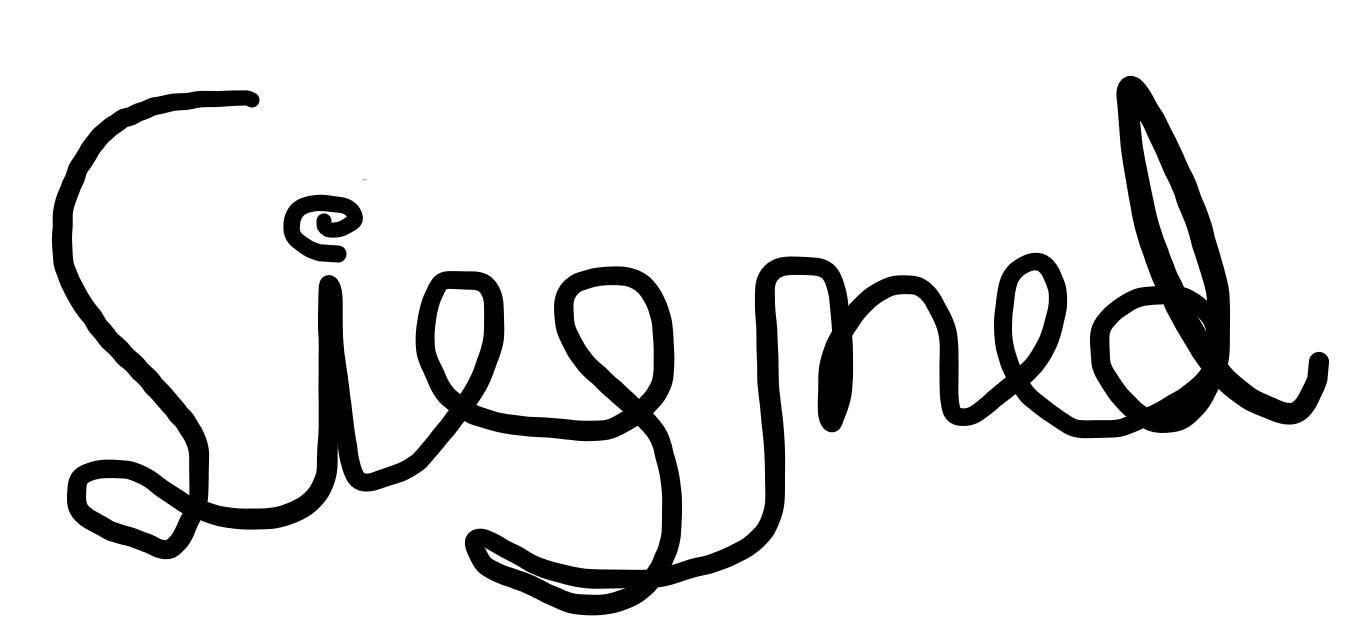
\includegraphics[height=2.5em,keepaspectratio]{Figures/SignatureMe.png}}%%
\hfill%%
\textbf{Date:} \today

I hereby certify that the above declaration correctly reflects the nature and extent of the student's and co-authors' contributions to this work. In instances where I am not the responsible author I have consulted with the responsible author to agree on the respective contributions of the authors.

%% ACTION: Add your main supervisor's name and signature file
\textbf{Main Supervisor name:} NAME

\textbf{Main Supervisor signature:}\hspace{3mm}%%
\raisebox{-.5\height}{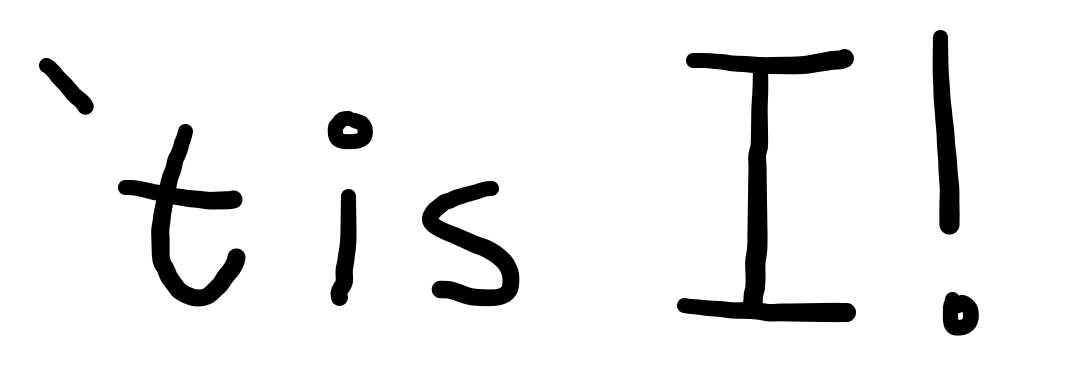
\includegraphics[height=2.5em,keepaspectratio]{Figures/SignatureSupervisor.png}}%%
\hfill%%
\textbf{Date:} \today


}
\clearpage  % Declaration ended, now start a new page




%% ----------------------------------------------------------------
% The Acknowledgements page, for thanking everyone
\setstretch{1.3}  % Reset the line-spacing to 1.3 for body text (if it has changed)
%% (REQUIRED)
%% ACTION
%%      Acknowledge your funding sources e.g. scholarships, grants
%%      The format of this section is mostly up to you. I have added a rough outline. You may alter this.
\ack{{}
Thank you to everyone who has supported me\footnote{\printThesisAuthor \href{https://orcid.org/0000-0000-0000-0000}{
\includegraphics[height=2ex]{Figures/ORCIDiD_iconvector.pdf} https://orcid.org/0000-0000-0000-0000}} during my candidature.

NAME\footnote{NAME \href{https://orcid.org/0000-0000-0000-0000}{
\includegraphics[height=2ex]{Figures/ORCIDiD_iconvector.pdf} https://orcid.org/0000-0000-0000-0000}} \textbf{---} My main supervisor. Thanks for being a great supervisor!

NAME\footnote{NAME \href{https://orcid.org/0000-0000-0000-0000}{
\includegraphics[height=2ex]{Figures/ORCIDiD_iconvector.pdf} https://orcid.org/0000-0000-0000-0000}} \textbf{---} My 2nd supervisor. Thanks for being a great supervisor!


This research was supported by an Australian Government Research Training Program (RTP) Scholarship.





}
\clearpage  % End of the Acknowledgements
%% ----------------------------------------------------------------

\pagestyle{fancy}  %The page style headers have been "empty" all this time, now use the "fancy" headers as defined before to bring them back


%% ----------------------------------------------------------------
\lhead{\emph{Contents}}  % Set the left side page header to "Contents"
\tableofcontents  % Write out the Table of Contents

%% ----------------------------------------------------------------
\lhead{\emph{List of Figures}}  % Set the left side page header to "List if Figures"
\listoffigures  % Write out the List of Figures

%% ----------------------------------------------------------------
\lhead{\emph{List of Tables}}  % Set the left side page header to "List of Tables"
\listoftables  % Write out the List of Tables

%% ----------------------------------------------------------------
\setstretch{1.5}  % Set the line spacing to 1.5, this makes the following tables easier to read
\clearpage  % Start a new page
\lhead{\emph{Abbreviations}}  % Set the left side page header to "Abbreviations"
\listofsymbols{ll}  % Include a list of Abbreviations (a table of two columns)
{
% \textbf{Acronym} & \textbf{W}hat (it) \textbf{S}tands \textbf{F}or \\
\textbf{LAH} & \textbf{L}ist \textbf{A}bbreviations \textbf{H}ere \\

}

%% ----------------------------------------------------------------
\clearpage  % Start a new page
\lhead{\emph{Constants}}  % Set the left side page header to "Physical Constants"
\listofconstants{lrcl}  % Include a list of Physical Constants (a four column table)
{
% Constant Name & Symbol & = & Constant Value (with units) \\
Speed of Light & $c$ & $=$ & $2.997\ 924\ 58\times10^{8}\ \mbox{ms}^{-2}$\\

}

%% ----------------------------------------------------------------
\clearpage  %Start a new page
\lhead{\emph{Symbols}}  % Set the left side page header to "Symbols"
\listofnomenclature{lll}  % Include a list of Symbols (a three column table)
{
% symbol & name & unit \\
$a$ & distance & m \\
$P$ & power & W (Js$^{-1}$) \\
& & \\ % Gap to separate the Roman symbols from the Greek
$\omega$ & angular frequency & rads$^{-1}$ \\
}
%% ----------------------------------------------------------------
% End of the pre-able, contents and lists of things


%% ----------------------------------------------------------------
\mainmatter	  % Begin normal, numeric (1,2,3...) page numbering
\pagestyle{fancy}  % Return the page headers back to the "fancy" style

% Include the chapters of the thesis, as separate files
% Just uncomment the lines as you write the chapters

\fancyhead{}  % Clears all page headers and footers
\rhead{\thepage}  % Sets the right side header to show the page number
\lhead{}  % Clears the left side page header
\chapter{Introduction}

\section{Writing a thesis}
Writing a thesis is a lengthy process, often requiring multiple redrafts and revisions.

Drafts should be provided and reviewed on a regular basis to keep up momentum as the submission deadline approaches. Please ensure that all required milestones and program requirements (e.g., professional development hours) have been completed before progressing with your submission.

The information below has been provided to you to make your experience as easy as possible. You may also like to refer to the Graduate Research Thesis Examination Procedures for further insight into the thesis examination process.

\subsection{What format the thesis will be presented}
The first thing to consider is in what format the thesis will be presented.
We recommend students and main supervisors discuss this as early as possible, and jointly agree on the most appropriate option:

Traditional thesis: A similar format to research reports and papers where the research question is proposed, methodology is described and the results are discussed and conclusions established.

Thesis including published works: Overall format is the same as a traditional thesis but particular chapters will include any submitted publications. Some Faculties have their own criteria for what can be included in this format.

All theses must use the approved thesis preliminary pages which includes compulsory information such as copyright and authorship declarations. If these pages are not presented correctly, the thesis will not be dispatched to the examiners and the relevant sections will need to be amended.

\subsection{Examiners}
At Monash each graduate research student has a supervisory team. Of this group, the main supervisor is responsible for approaching potential examiners for their students' thesis. Initial discussions normally take place at the student's final milestone review and it is recommended that examiners are approached at least 4-6 weeks before expected submission.

An email template is available for use when inviting potential examiners to examine a thesis.

For students enrolled in a Live Music or Theatre Performance degree, the main supervisor will also need to complete a Nomination of Examiners form. This form will require the approval of the Program Director (or delegate) and the Monash Graduate Research Office prior to the live performance. For further information please contact the Faculty of Arts.

In addition, when considering appropriate examiners, please note that if an examiner is subject to Sanctions laws, we are unable to provide payment for their thesis examination.

\subsection{Conflict of interest}
There are a range of circumstances that could result in a conflict of interest, potentially restricting the objectivity of the examiners.

Some examples of what we consider conflicts of interest are:
\begin{itemize}
\item Involvement in the student's research, including supervision of the candidate in field or laboratory work or elsewhere during candidature.
\item Previous work in the same department within an institution as the candidate.
\item A previous appointment as an academic staff member at Monash University, including an adjunct academic appointment, during the student’s period of candidature.
\item Holding the position of emeritus or adjunct professor at Monash.
\item Substantial contact with the candidate in any other circumstance which might jeopardise the independence of the examination.
\item Being a close associate (spouse/partner, other relative, friend or business partner) of either the candidate or the supervisor of the candidate.
\end{itemize}
There is a more comprehensive list of grounds for conflicts of interest which you may wish to review.


\section{Thesis including Published Works}
All doctoral and research master's students are permitted to submit a thesis including published works, in accordance with section 1.9 of the Graduate Research Thesis Examination Procedures. The thesis including published works is not a different degree; rather, it is a thesis format that includes papers that have been submitted, or accepted, for publication, during the course of the student's enrolment in the relevant graduate research degree at Monash.

The thesis must reflect a sustained and cohesive theme, and framing or substantial linking text is normally required in introducing the research and linking the chapter/papers/manuscripts. The papers do not have to be rewritten for the thesis. For guidance, refer to Text Framing the Publications (as below).

Whether the papers are required to have been published, accepted for publication, or only submitted for publication varies across faculties (see Faculty Requirements below). We advise you to consult good examples of theses including published works in your discipline. Your academic unit or school should have copies of all doctoral and research master's theses available for consultation. Workshops on the thesis including published works are also run through the Skills Essentials series, if you require more information.


\section{The maximum word length}
For references see \href{http://www.monash.edu/__data/assets/pdf_file/0011/911882/Graduate-Research-Thesis-Examination-Procedures.pdf}{Graduate Research Thesis Examination Procedures} 

PhD: 80,000 words,  100,000 words for students enrolled prior to 1 January 2015

MPhil: 35,000 words, 50,000 words for students enrolled prior to 1 January 2015.

\section{Using Figures and Tables, and other commands}

We have defined several commands in thesis.cls file for easier usage:
\begin{verbatim}
\newcommand{\fref}[1]{Figure~\ref{#1}}
\newcommand{\tref}[1]{Table~\ref{#1}}
\newcommand{\eref}[1]{Equation~\ref{#1}}
\newcommand{\cref}[1]{Chapter~\ref{#1}}
\newcommand{\sref}[1]{Section~\ref{#1}}
\newcommand{\aref}[1]{Appendix~\ref{#1}}
\renewcommand{\topfraction}{0.85}
\renewcommand{\bottomfraction}{.85}
\renewcommand{\textfraction}{0.1}
\renewcommand{\dbltopfraction}{.85}
\renewcommand{\floatpagefraction}{0.75}
\renewcommand{\dblfloatpagefraction}{.75}
\end{verbatim}

You can use \textit{fref} and \textit{tref} to refer a figure and table, such as \fref{fig.demo1} and \tref{table.demo1}. Refer a citation like this \cite{Reference1}. You can cite multiple references once, like this \cite{Reference1,Reference2,Reference3}.



\begin{figure}
\centering
  
\includegraphics[height=5cm]{Figures/crest.jpg}%
  \caption{My Picture Demo\label{fig.demo1}}
\end{figure}

\begin{table}[]
\caption{Table Demo.\label{table.demo1}}
\centering
\begin{tabular}{|c|c|c|}
\hline
Description & Images &  \\ \hline
Training & Taking 3 knowns + 1 known unknown randomly & 2900 \\ \hline
Gallery & Taking 3 images of knowns randomly & 1830 \\ \hline
Probe C & C=S & 4903 \\ \hline
Probe O1 & O1 & 6264 \\ \hline
Probe O2 & O2 & 8972 \\ \hline
Probe O3 & O3 & 10333 \\ \hline
\end{tabular}
\end{table}

\section{A Section}

Quisque tristique urna in lorem laoreet at laoreet quam congue. Donec dolor turpis, blandit non imperdiet aliquet, blandit et felis. In lorem nisi, pretium sit amet vestibulum sed, tempus et sem. Proin non ante turpis. Nulla imperdiet fringilla convallis. Vivamus vel bibendum nisl. Pellentesque justo lectus, molestie vel luctus sed, lobortis in libero. Nulla facilisi. Aliquam erat volutpat. Suspendisse vitae nunc nunc. Sed aliquet est suscipit sapien rhoncus non adipiscing nibh consequat. Aliquam metus urna, faucibus eu vulputate non, luctus eu justo.

\subsection{A Subsection}

Donec urna leo, vulputate vitae porta eu, vehicula blandit libero. Phasellus eget massa et leo condimentum mollis. Nullam molestie, justo at pellentesque vulputate, sapien velit ornare diam, nec gravida lacus augue non diam. Integer mattis lacus id libero ultrices sit amet mollis neque molestie. Integer ut leo eget mi volutpat congue. Vivamus sodales, turpis id venenatis placerat, tellus purus adipiscing magna, eu aliquam nibh dolor id nibh. Pellentesque habitant morbi tristique senectus et netus et malesuada fames ac turpis egestas. Sed cursus convallis quam nec vehicula. Sed vulputate neque eget odio fringilla ac sodales urna feugiat.

\section{Another Section}

Phasellus nisi quam, volutpat non ullamcorper eget, congue fringilla leo. Cras et erat et nibh placerat commodo id ornare est. Nulla facilisi. Aenean pulvinar scelerisque eros eget interdum. Nunc pulvinar magna ut felis varius in hendrerit dolor accumsan. Nunc pellentesque magna quis magna bibendum non laoreet erat tincidunt. Nulla facilisi.

Duis eget massa sem, gravida interdum ipsum. Nulla nunc nisl, hendrerit sit amet commodo vel, varius id tellus. Lorem ipsum dolor sit amet, consectetur adipiscing elit. Nunc ac dolor est. Suspendisse ultrices tincidunt metus eget accumsan. Nullam facilisis, justo vitae convallis sollicitudin, eros augue malesuada metus, nec sagittis diam nibh ut sapien. Duis blandit lectus vitae lorem aliquam nec euismod nisi volutpat. Vestibulum ornare dictum tortor, at faucibus justo tempor non. Nulla facilisi. Cras non massa nunc, eget euismod purus. Nunc metus ipsum, euismod a consectetur vel, hendrerit nec nunc. % Introduction

% the following chapter shows how to include an external pdf as a chapter after a preamble page.
\chapter{Including a published pdf as a thesis chapter}

In a thesis including published works, some chapters may simply involve including an external (published) \texttt{.pdf} file into your thesis document.

The following sample shows how to insert a subset of pages of a \texttt{.pdf} in such a way that the page numbering of the thesis is also added to the included \texttt{.pdf} pages. 
It also scales and translates the inserted \texttt{.pdf} file to fit within the margins of the thesis. 

% In the following command: 
% -- the argument {external} is the path to the pdf you would like to include (here the file happens to be called external.pdf and is in the Figures folder)
% -- the optional argument pages=1-2 inserts pages 1-2 of the referenced pdf (change this as required, for all pages write pages={-})
% -- the optional argument pagecommand={} keeps the overall page formatting of the thesis, including the overall page numbering
% -- the optional argument scale=0.85 scales the included pdf so it fits nicely on the thesis page (this may need to be altered depending on the margins of the pdf)
% -- the optinal argument offset=<x offset>mm <yoffset>mm specifies an offset from the nominal position. This will need to be adjusted so that the included document is placed well on the thesis page (i.e., margins are not violated, etc). In the example, the page is shifted 30mm to the right, and 20mm down (i.e., -20mm vertical offset). 
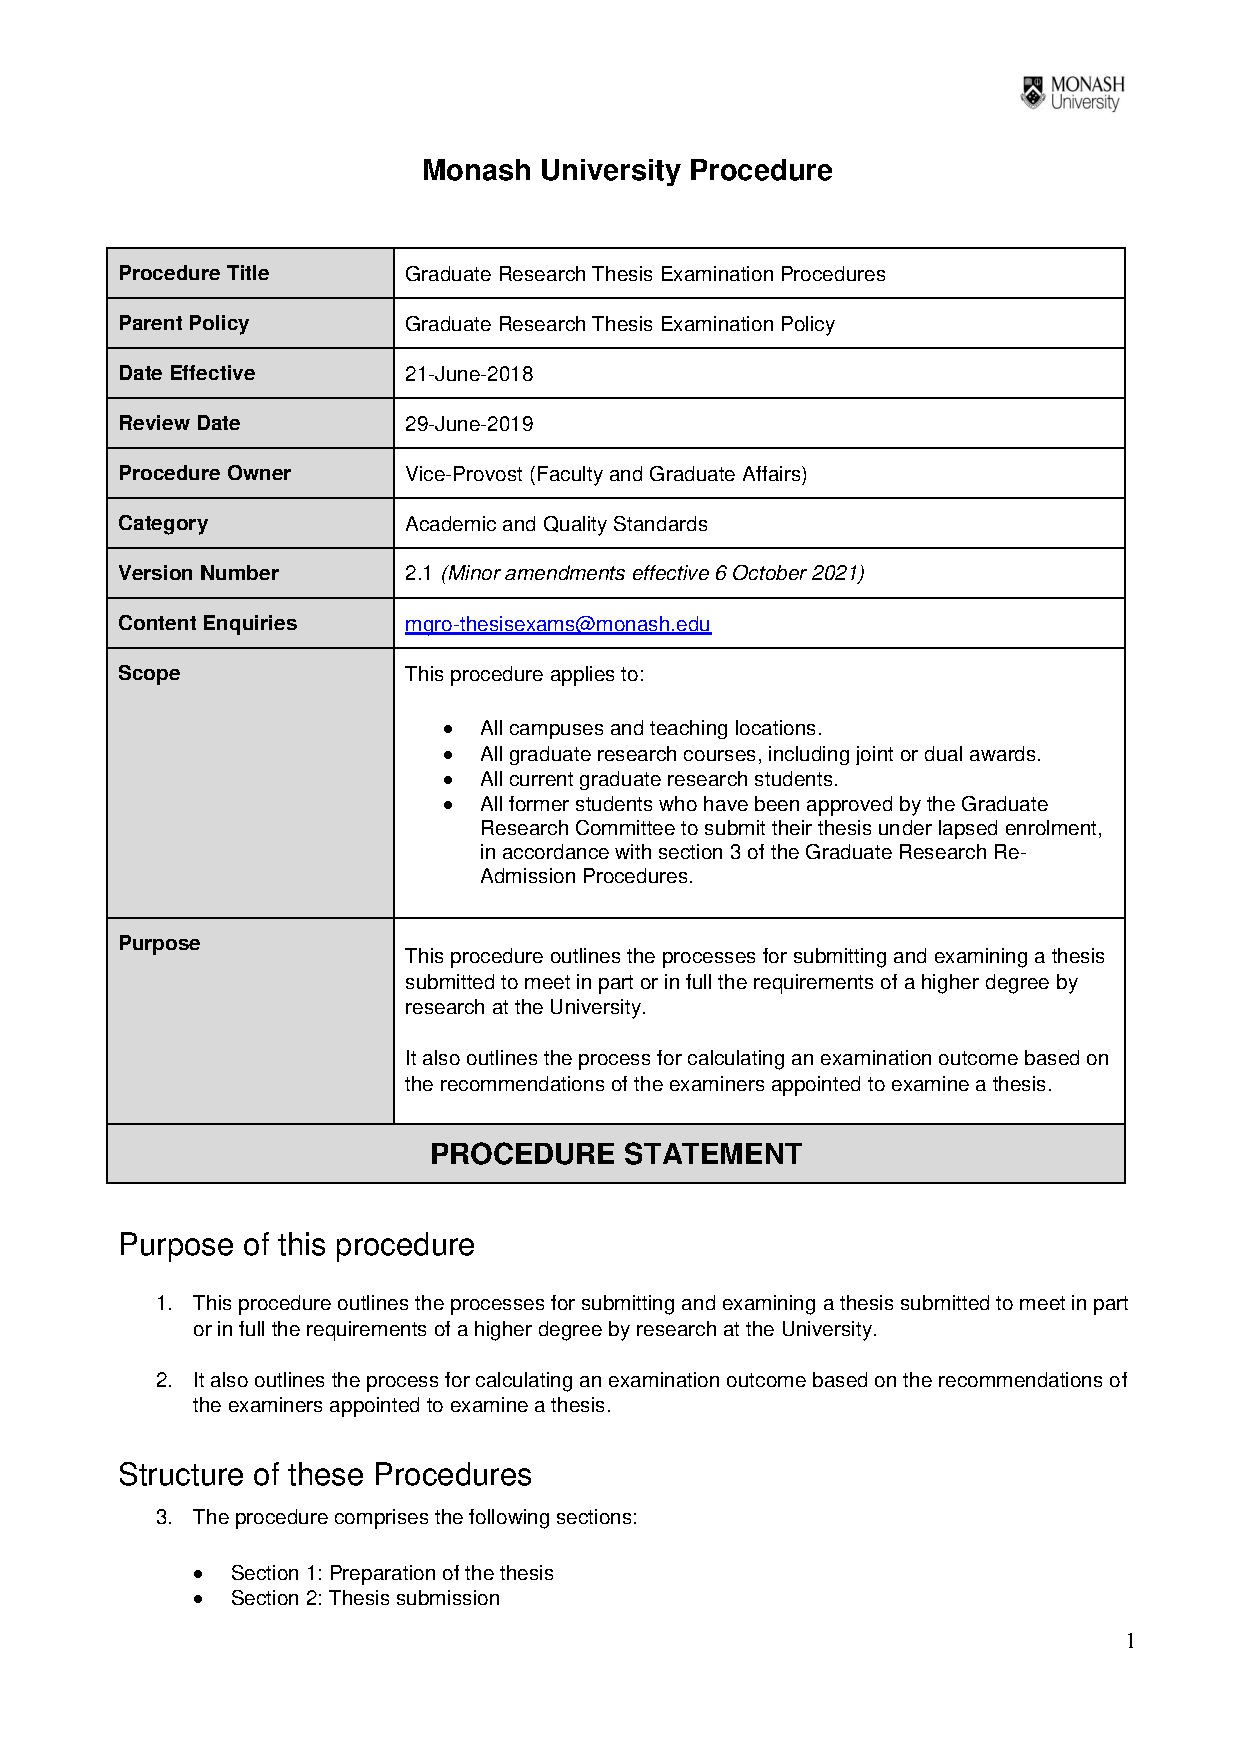
\includepdf[pages=1-2,pagecommand={},scale=0.85,offset=30mm -20mm]{Figures/external} 

%\chapter{My First Published Article} \label{chap:article1}
\begin{displayquote} \emph{%%
	This chapter embeds a copy of my publication \cite{example3}, which is distributed under the \href{https://creativecommons.org/licenses/by/4.0/}{Creative Commons CC BY 4.0 license}.
} \end{displayquote}

%% Intro & link to objectives



%%%%%%%%%%%%%%%%%%%%%%%%%%%%%%%%%%%%%%%%%%%%%%%%%%%%%%%%%%%%%%%%%%%%%%%%%%%%%%%%%
%%%%%%%%%%%%%%%%%%%%%%%%%%%%%%%%%%%%%%%%%%%%%%%%%%%%%%%%%%%%%%%%%%%%%%%%%%%%%%%%%
\section{The Title of My First Published Article}
List of Amendments to \cite{example3}
\begin{itemize}[topsep=0pt,beginpenalty=10000,first=\interlinepenalty10000]
	\item Equation 6 contains a typographical error, in which ${}^O\text{\textbf{p}}_i$ should be ${}^O\dot{\text{\textbf{p}}}_i$
\end{itemize}

%% The following embedded document represents your published article.
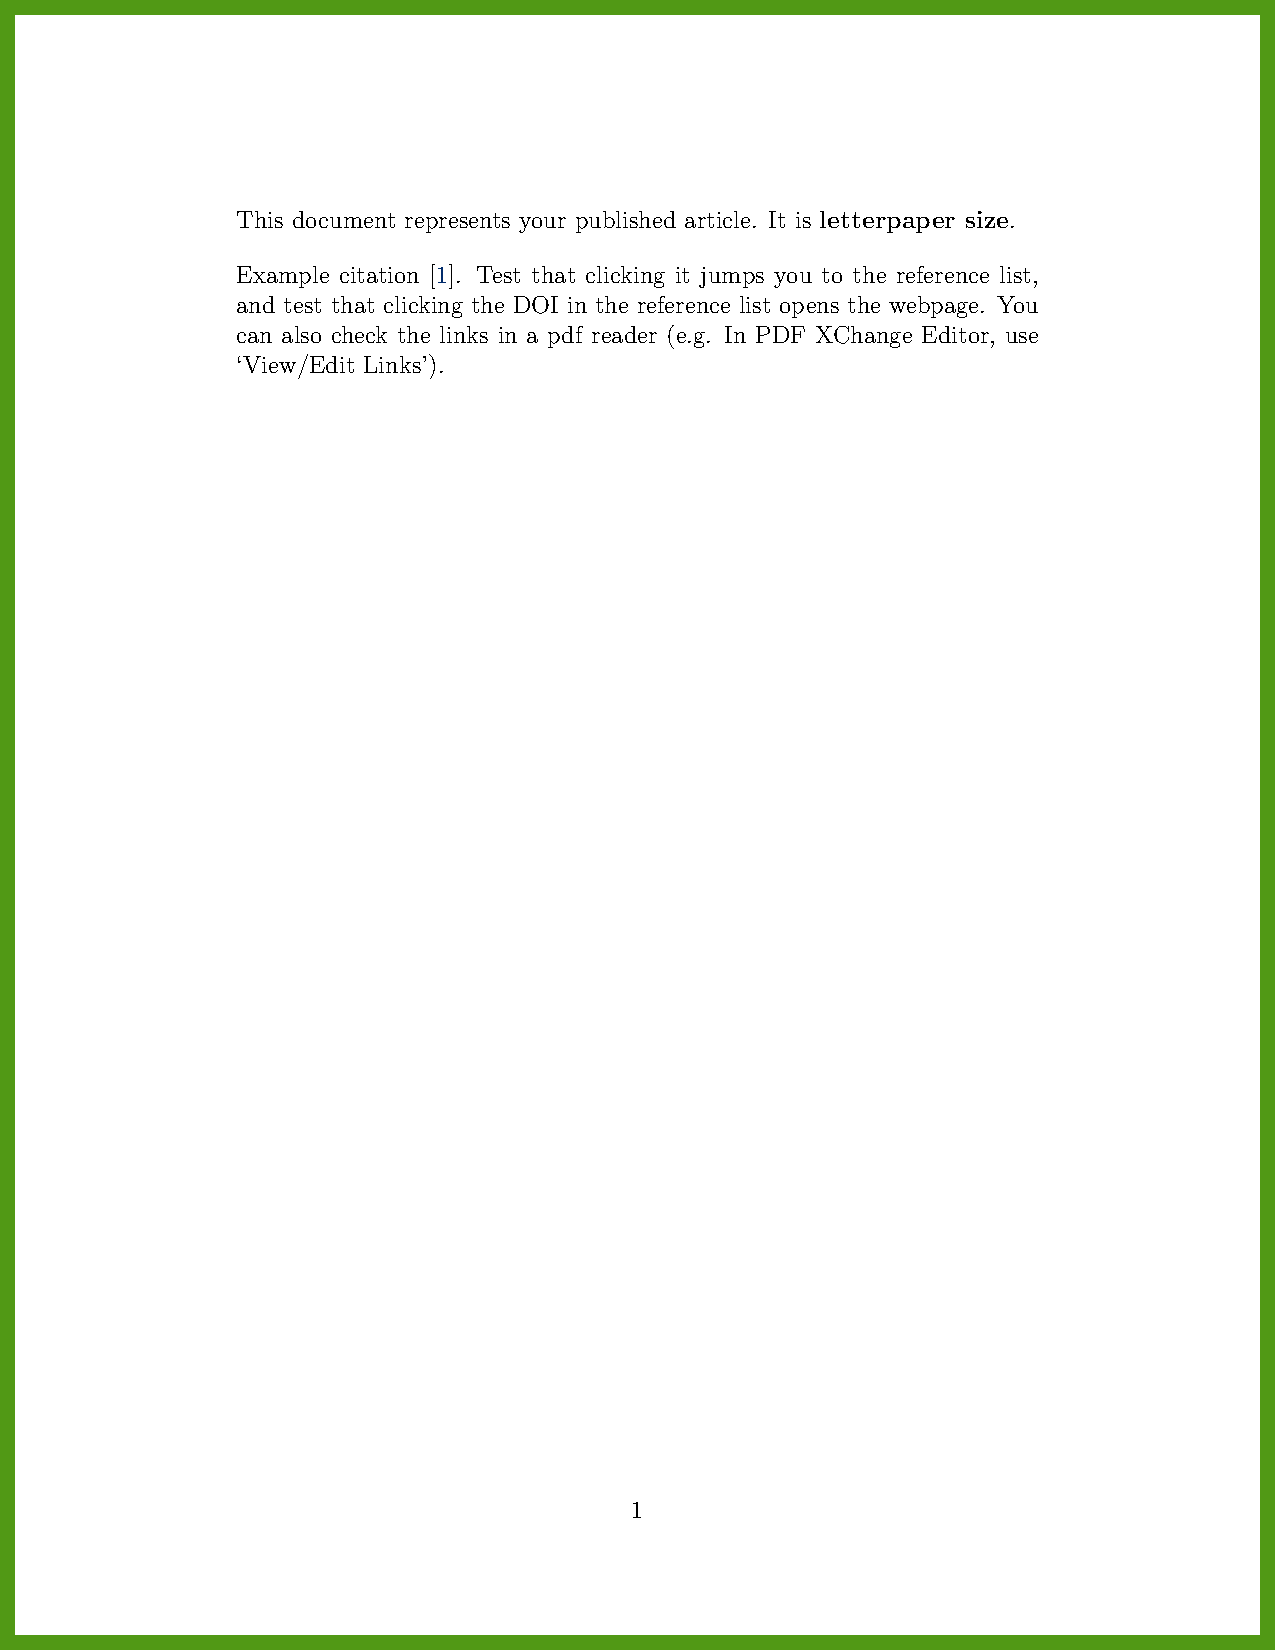
\includepdf[pages={-},pagecommand={},offset=0mm 10mm]{MyPublishedArticle1.pdf}

%% NOTE 1
%% The article is being embedded into an A4 document.
%% If the article is not A4, then it will be shrunk to fit and centred in the page.
%% The offset parameter can move from the default position
%% => If the thesis footer overlaps the included pdf, then try changing the scale and offset
%% e.g.
%% 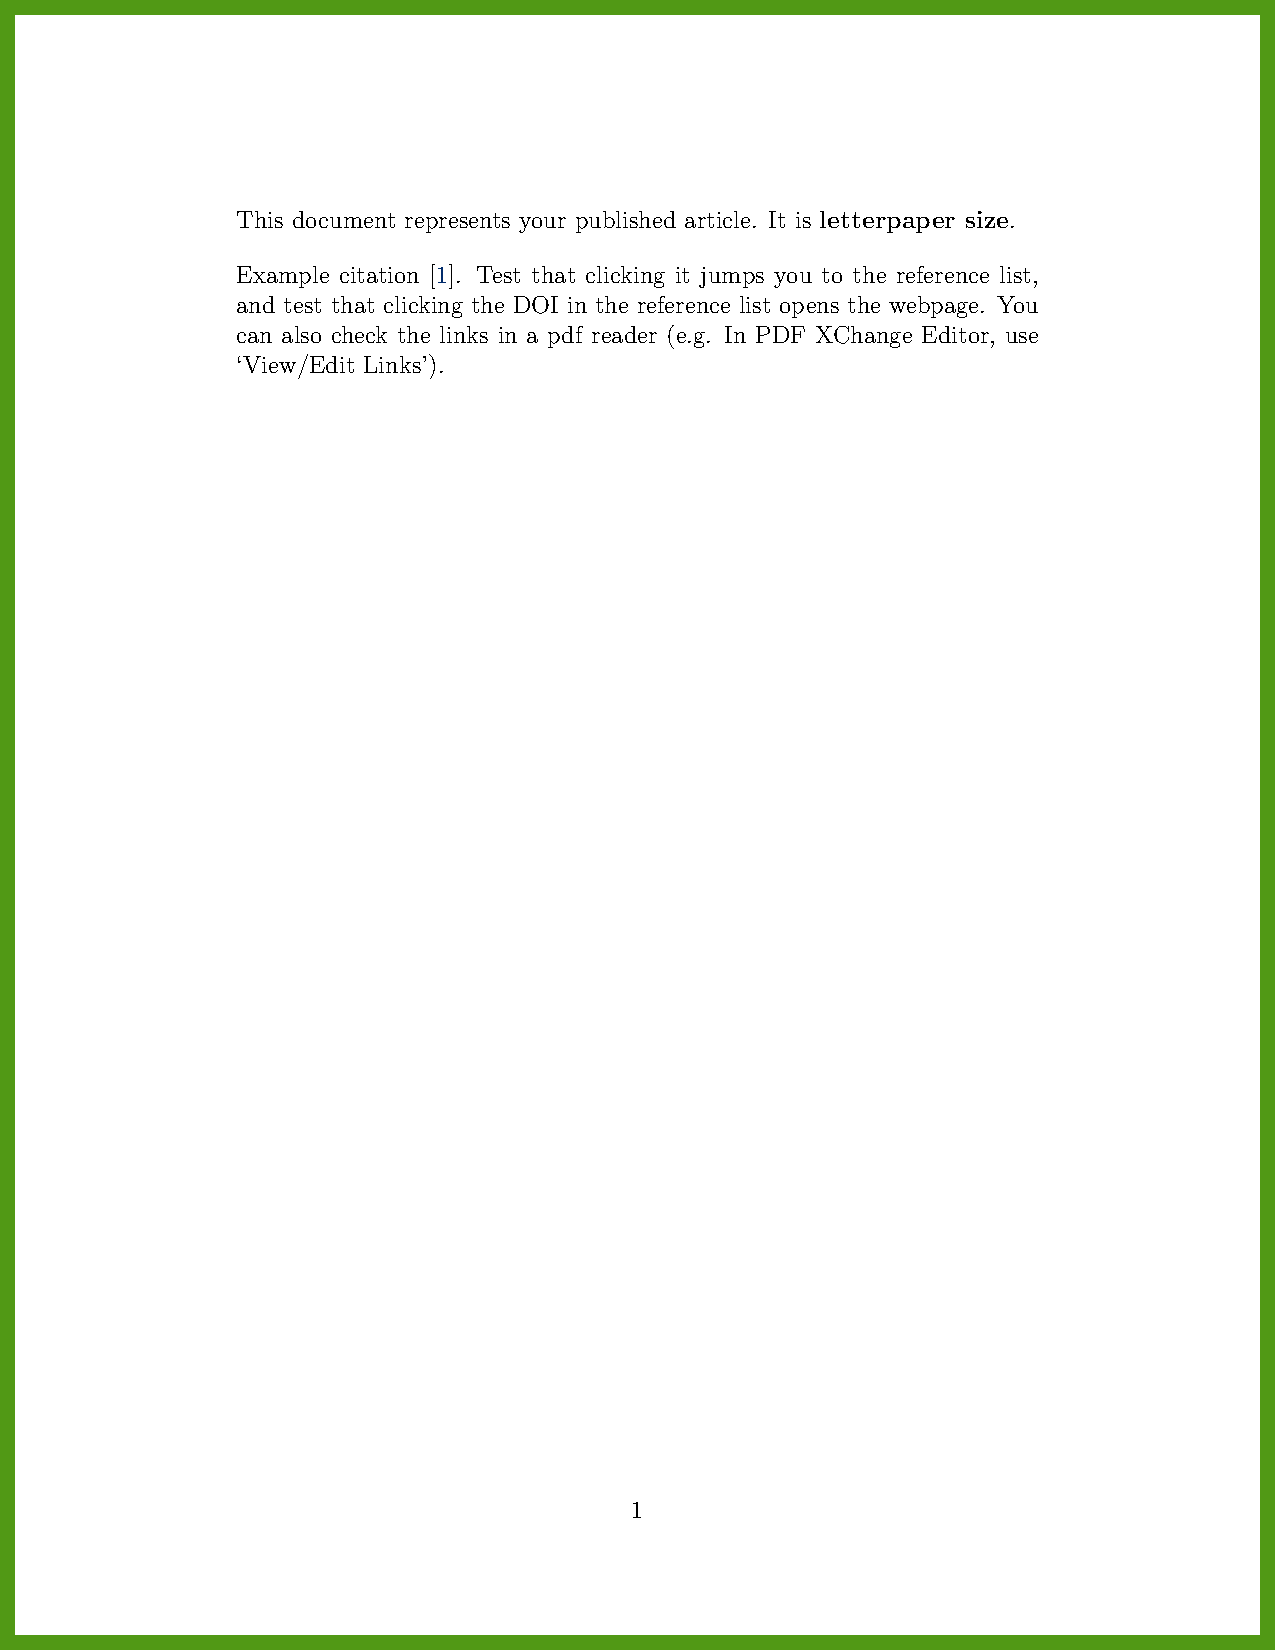
\includepdf[pages={-},pagecommand={},scale=0.95,offset=0mm 5mm]{MyPublishedArticle1.pdf}

%% NOTE 2
%% By using the package `pdfpages' to embed this pdf into the thesis, all the hyperlinks become no longer clickable.
%% To reinsert the links, the package `pax' can be used
%% Reinserting the links requires some manual work, and the `pax' is not flawless.
%% Follow the instructions in Thesis.tex, and be sure to test that it works.


%%%%%%%%%%%%%%%%%%%%%%%%%%%%%%%%%%%%%%%%%%%%%%%%%%%%%%%%%%%%%%%%%%%%%%%%%%%%%%%%%
%%%%%%%%%%%%%%%%%%%%%%%%%%%%%%%%%%%%%%%%%%%%%%%%%%%%%%%%%%%%%%%%%%%%%%%%%%%%%%%%%
\section{Outlook}
%% Link results to objectives
The outcomes of this work ...

The work finds that ...

The next chapter applies these results to ...

 

%\chapter{My Second Published Article} \label{chap:article2}
\begin{displayquote} \emph{%%
	This chapter embeds a copy of my publication \cite{example5}, which is distributed under the \href{https://creativecommons.org/licenses/by/4.0/}{Creative Commons CC BY 4.0 license}.
} \end{displayquote}

%% Intro & link to objectives



%%%%%%%%%%%%%%%%%%%%%%%%%%%%%%%%%%%%%%%%%%%%%%%%%%%%%%%%%%%%%%%%%%%%%%%%%%%%%%%%%
%%%%%%%%%%%%%%%%%%%%%%%%%%%%%%%%%%%%%%%%%%%%%%%%%%%%%%%%%%%%%%%%%%%%%%%%%%%%%%%%%
\section{The Title of My Second Published Article}
%% If the footer overlaps the included pdf, then try changing the scale and offset options e.g.
%% 
\includepdf[pages={-},pagecommand={},scale=0.95,offset=0mm 5mm]{MyPublishedArticle2.pdf}


\includepdf[pages={-},pagecommand={}]{MyPublishedArticle2.pdf}


%%%%%%%%%%%%%%%%%%%%%%%%%%%%%%%%%%%%%%%%%%%%%%%%%%%%%%%%%%%%%%%%%%%%%%%%%%%%%%%%%
%%%%%%%%%%%%%%%%%%%%%%%%%%%%%%%%%%%%%%%%%%%%%%%%%%%%%%%%%%%%%%%%%%%%%%%%%%%%%%%%%
\section{Outlook}
%% Link results to objectives
The outcomes of this work ...


 

%\chapter{Conclusions and Outlook} \label{chap:conclusions}
%% Scope / Motivations / Problem Statement

%% Aims
%% Contributions as dot points
This thesis contributes to ... The key contributions are:
\begin{itemize}[topsep=0pt,beginpenalty=10000,first=\interlinepenalty10000]
	\item Something
	\item Something
	\item Something
\end{itemize}

%% Results and outlook
The outcomes of this work ...:
\begin{itemize}[topsep=0pt,beginpenalty=10000,first=\interlinepenalty10000]
	\item In \chapref{chap:article1}, it is found that ...
	\item In \chapref{chap:article2}, ...
\end{itemize}

%% Directions
Future work is recommended to ... Specific directions for future work are:
\begin{itemize}[topsep=0pt,beginpenalty=10000,first=\interlinepenalty10000]
	\item Something
	\item Something
	\item Something
\end{itemize}

 

%\input{Chapters/Chapter6} 

%\input{Chapters/Chapter7} 

%% ----------------------------------------------------------------
% Now begin the Appendices, including them as separate files

\addtocontents{toc}{\vspace{2em}} % Add a gap in the Contents, for aesthetics

\appendix % Cue to tell LaTeX that the following 'chapters' are Appendices

\chapter{An Appendix}
Example text.

%%%%%%%%%%%%%%%%%%%%%%%%%%%%%%%%%%%%%%%%%%%%%%%%%%%%%%%%%%%%%%%%%%%%%%%%%%%%%%%%%
%%%%%%%%%%%%%%%%%%%%%%%%%%%%%%%%%%%%%%%%%%%%%%%%%%%%%%%%%%%%%%%%%%%%%%%%%%%%%%%%%
\section{Displaying Sections}
Example text.

\clearpage

%%%%%%%%%%%%%%%%%%%%%%%%%%%%%%%%%%%%%%%%%%%%%%%%%%%%%%%%%%%%%%%%%%%%%%%%%%%%%%%%%
\subsection{My Subsection}
Example text.


%%%%%%%%%%%%%%%%%%%%%%%%%%%%%%%%%%%%%%%%%%%%%%%%%%%%%%%%%%%%%%%%%%%%%%%%%%%%%%%%%
\subsubsection{My Subsubsection}
Example text.

\clearpage

%%%%%%%%%%%%%%%%%%%%%%%%%%%%%%%%%%%%%%%%%%%%%%%%%%%%%%%%%%%%%%%%%%%%%%%%%%%%%%%%%
\paragraph{My Subsubsubsection... WAIT WHAT!?}
If you get this deep, the command is not `subsubsubsection', but `paragraph'. Why?

For the record, I really suggest not to use this much depth unless you've really thought about your structure, and you are sure that it is the best way to do it.

%%%%%%%%%%%%%%%%%%%%%%%%%%%%%%%%%%%%%%%%%%%%%%%%%%%%%%%%%%%%%%%%%%%%%%%%%%%%%%%%%
\subparagraph{My Subsubsubsubsection... rofl}
This is the maximum section depth that the titlesec package allows. May you never need it.


%%%%%%%%%%%%%%%%%%%%%%%%%%%%%%%%%%%%%%%%%%%%%%%%%%%%%%%%%%%%%%%%%%%%%%%%%%%%%%%%%
\subsection{My Other Subsection}
Example text.

	% Appendix Title

%\chapter{Another Appendix}
todo
 % Appendix Title

%\input{Appendices/AppendixC} % Appendix Title

\addtocontents{toc}{\vspace{2em}}  % Add a gap in the Contents, for aesthetics
\backmatter

%% ----------------------------------------------------------------
\label{Bibliography}
\lhead{\emph{Bibliography}}  % Change the left side page header to "Bibliography"
\bibliographystyle{unsrtnat}  % Use the "unsrtnat" BibTeX style for formatting the Bibliography
\bibliography{Bibliography}  % The references (bibliography) information are stored in the file named "Bibliography.bib"

\end{document}  % The End
%% ----------------------------------------------------------------